% Created 2015-06-01 ma. 17:42
\documentclass[11pt]{article}
\usepackage[utf8]{inputenc}
\usepackage[T1]{fontenc}
\usepackage{fixltx2e}
\usepackage{graphicx}
\usepackage{longtable}
\usepackage{float}
\usepackage{wrapfig}
\usepackage{rotating}
\usepackage[normalem]{ulem}
\usepackage{amsmath}
\usepackage{textcomp}
\usepackage{marvosym}
\usepackage{wasysym}
\usepackage{amssymb}
\usepackage{capt-of}
\usepackage{hyperref}
\tolerance=1000
\usepackage{minted}
\usepackage{color}
\usepackage{listings}
\usepackage{grffile}
\definecolor{mintedbackground}{rgb}{0.95,0.95,0.95}
\usepackage[inline]{enumitem}
\usepackage{xcolor}
\hypersetup{
colorlinks,
linkcolor={red!50!black},
citecolor={blue!50!black},
urlcolor={blue!80!black}
}
\usepackage{tikz,graphics,graphicx}
\usetikzlibrary{decorations.shapes,arrows,decorations.pathreplacing,decorations.pathmorphing,backgrounds}
\usetikzlibrary{decorations.pathmorphing}
\usetikzlibrary{shapes.geometric}
\usepackage{setspace}%% The linestretch
\singlespacing
\usepackage[format=hang,indention=0cm,singlelinecheck=true,justification=raggedright,labelfont={normalsize,bf},textfont={normalsize}]{caption} %
\usepackage{vmargin}
\setpapersize{A4}
\setmarginsrb{2.5cm}{1cm}% links, oben
{2.5cm}{2cm}% rechts, unten
{12pt}{30pt}% Kopf: Höhe, Abstand
{12pt}{30pt}% Fuß: Höhe, AB
\usepackage{upquote}
%  use straight quotes when printing a command in minted
\AtBeginDocument{%
\def\PYZsq{\textquotesingle}%
}
\setlength{\parindent}{0pt}
\setlength{\parskip}{\baselineskip}
\definecolor{mintedbackground}{rgb}{0.95,0.95,0.95}
\author{Alexander Jueterbock, Martin Jakt\thanks{University of Nordland, Norway}}
\date{\textbf{PhD course: High throughput sequencing of non-model organisms}}
\title{\textbf{Mapping and Variant Calling} (2015-06-04)}
\hypersetup{
 pdfkeywords={},
  pdfsubject={},
  pdfcreator={Emacs 24.3.1 (Org mode 8.3beta)}}
\begin{document}

\maketitle
\tableofcontents







Once you have assembled a draft genome, you can map your reads against it
and identify potential read variants, like SNPs (Single Nucleotide
Polymorphisms) and InDels (Insertions and Deletions). The library that
you sequenced in this course is likely to represent a single diploid
individual. Read variants, thus, occur at loci that differed between
the mother and the father of this individual. Read variants become
interesting when they are associated with certain environmental
factors or phenotypes. This, however, requires sequencing several
individuals of differing phenotypes or obtained from several  
environments.

\section{Mapping with Bowtie2}
\label{sec-1}
To map reads against the assembled draft genome, we will use \href{http://bowtie-bio.sourceforge.net/bowtie2/index.shtml}{Bowtie2}.
Bowtie2 defaults to finding global alignments (no soft-clipping of
terminal bases) and it allows for gaps in the alignment, thereby
increasing mapping accurracy (\href{http://www.nature.com/nrg/journal/v15/n11/full/nrg3803.html}{Schlotterer \emph{et al}. (2014) \emph{Nature
Reviews Genetics}}). Although the aligner \href{https://www.google.no/url?sa=t&rct=j&q=&esrc=s&source=web&cd=5&ved=0CD4QFjAE&url=https\%3A\%2F\%2Fgithub.com\%2Fiontorrent\%2FTMAP&ei=1u07VZCXFYGqywPBz4DoDg&usg=AFQjCNE3vZXuQ1ygljhBcrozKj_nBU84TQ&sig2=u5_YVYBE904ay-9oLUuMOQ&bvm=bv.91665533,d.bGQ}{TMAP} was specifically
compiled for Ion Torrent data, in this tutorial we want use an aligner
that can also be used with Illumina or SoliD data - as you are likely
to work with sequencing data that were obtained from these
platforms in the future. An alternative aligner that is currently widely used is
\href{http://bio-bwa.sourceforge.net/}{BWA}.

What you need for mapping are two fasta files, one containing the
quality-trimmed reads and the other containing the draft genome.
Create a new folder named \texttt{Mapping} (with \texttt{mkdir}) and copy the two
fasta files into it (with \texttt{cp}). For example:

\begin{minted}[fontsize=\scriptsize,bgcolor=lightgray,linenos]{sh}
mkdir Mapping

cp GenomeAssembly/IonTorrentDeNovoAssembly_d_results/\
IonTorrentDeNovoAssembly_out.unpadded.fasta \
Mapping/

cp RAWREADS_trimmed_trimmed.fq \
Mapping/

cd Mapping
\end{minted}


In the Mapping folder, we first create an index for the reference genome using the
following command:

\begin{minted}[fontsize=\scriptsize,bgcolor=lightgray,linenos]{sh}
bowtie2-build -f IonTorrentDeNovoAssembly_out.unpadded.fasta GENOMENAME
\end{minted}

You can change \texttt{GENOMENAME} to whatever you like.

Now, to align the trimmed reads against the genome, use the following command:

\begin{minted}[fontsize=\scriptsize,bgcolor=lightgray,linenos]{sh}
nohup bowtie2 -p 1 \
-q \
--phred33 \
--sensitive \
--no-unal \
--al-gz FILE_Aligned.fq.gz \
--un-gz FILE_Unaligned.fq.gz \
--met-file MetricsFile.txt \
-x GENOMENAME \
-U RAWREADS_trimmed_trimmed.fq \
-S MAPPEDREADS.sam >Logfile.log &
\end{minted}

Here an overview of the meaning of the used options:


\begin{description}
\item[{\texttt{-p 1}}] Causes Bowtie 2 to use a single thread.
Depending on the number of users and libraries we will  probably increase this.
\item[{\texttt{-q}}] Informs the program that the reads to map are saved in fastq files.
\item[{\texttt{-{}-phred33}}] Sets the quality encoding of the fastq files to  "Phred+33".
\item[{\texttt{-{}-sensitive}}] sets several options at once regarding the seeding and other adjustments.
\item[{\texttt{-{}-no-unal}}] Suppress SAM records for reads that do not align.
\item[{\texttt{-{}-al-gz}}] Write unpaired reads that align at least once to to the specified file.
\item[{\texttt{-{}-un-gz}}] Write unpaired reads that failed to align to the specified file.
\item[{\texttt{-{}-met-file}}] Write bowtie2 metrics to Metricsfile.txt.
\item[{\texttt{-x}}] Specifies the name of the genome.
\item[{\texttt{-U}}] Specify the unpaired reads to align (can contain a comma-separated list of several fq files).
\item[{\texttt{-S}}] Specify the sam file to which the alignment shall be saved.
\end{description}

You can't set the exact number of mismatches in the seed, but you can
adjust the mismatch penalty.  

The program should run no longer than 10-20 mins. The resulting output file will be
in the SAM format. For a detailed description of this format, see \href{https://samtools.github.io/hts-specs/SAMv1.pdf}{here}.

\section{Filter mappings}
\label{sec-2}
To remove unmapped reads, reads below a mapping quality of 20, and
reads that were not aligned uniquely (reads that were mapped to >1
places in the genome), use the python script \href{http://marinetics.org/2015/03/03/Bowtie2Filtering.html}{Bowtie2Filtering.py}:

\begin{minted}[fontsize=\scriptsize,bgcolor=lightgray,linenos]{sh}
Bowtie2Filtering.py -mq -u -a -s MAPPEDREADS.sam
\end{minted}

Your filtered reads will be saved in \texttt{MAPPEDREADSfiltered.sam}

Alternatively, you can 
use \href{http://samtools.sourceforge.net/samtools.shtml#mpileup}{samtools} to filter out reads with a mapping quality <20:

\begin{minted}[fontsize=\scriptsize,bgcolor=lightgray,linenos]{sh}
samtools view -Sh -q 20 -o MAPPEDREADS_QualityAbove20.sam MAPPEDREADS.sam
\end{minted}

Options:

\begin{description}
\item[{\texttt{-S}}] Input is in the sam format
\item[{\texttt{-h}}] Include the samfile header in the output
\item[{\texttt{-q}}] Skip alignments with a mapping quality below 20
\end{description}

\subsection{Removing duplicate reads}
\label{sec-2-1}
After quality-trimming, we counted the fraction of duplicate
reads. Duplicate reads have the same start and end
coordinates and map to the same region. Duplicates result from primer
or PCR bias towards these reads. As they can skew genotype estimates,
they should be removed before SNP calling.

To remove duplicates, we will use 'MarkDuplicates' from the \href{https://broadinstitute.github.io/picard/command-line-overview.html}{Picard
command line tools}. An alternative tool is \href{http://samtools.sourceforge.net/samtools.shtml}{samtools} rmdup, which
considers single-end reads to be duplicates when their mapping
locations are the same - even if the base composition differs between
the reads.

First, we need to convert our sam file to a bam file (a binary,
compressed version of a sam file that is not human-readable) and sort
the reads by the leftmost mapping coordinates.

\begin{minted}[fontsize=\scriptsize,bgcolor=lightgray,linenos]{sh}
samtools view -bSh MAPPEDREADS.sam  > MAPPEDREADS.bam
samtools sort MAPPEDREADS.bam MAPPEDREADS_sorted
\end{minted}

Meaning of the options:
\begin{description}
\item[{\texttt{-b}}] output in bam format
\item[{\texttt{-S}}] input in sam format
\item[{\texttt{-h}}] include the header in the output
\end{description}



Then, you can use the java script 'MarkDuplicates.jar' from Picard
tools to remove the duplicates from the sorted bam file:

\begin{minted}[fontsize=\scriptsize,bgcolor=lightgray,linenos]{sh}
picard-tools MarkDuplicates \
INPUT=MAPPEDREADS_sorted.bam \
OUTPUT=MAPPEDREADS_dedup.bam \
METRICS_FILE=MAPPED_metricsfile \
ASSUME_SORTED=true \
VALIDATION_STRINGENCY=SILENT \
REMOVE_DUPLICATES=true
\end{minted}

Duplication metrics will be written to the \texttt{MAPPED\_metricsfile}.


\subsection{Re-alignment around indels}
\label{sec-2-2}
Reads that are spanning InDels are often misaligned and can result in
false SNPs (see \href{http://www.nature.com/nrg/journal/v15/n11/full/nrg3803.html}{Schlotterer \emph{et al}. (2014) \emph{Nature Reviews
Genetics}}). These reads should be removed or re-aligned. We have not
enough time to re-align the reads in this course but the required
steps (using \href{https://www.broadinstitute.org/gatk/}{GATK}) are described in detail here:
\url{http://sfg.stanforde.edu/SFG.pdf}.

\section{Visualizing alignments}
\label{sec-3}
\subsection{Samtools tview: command-line viewer}
\label{sec-3-1}
The command line tool samtools tview allows you to view your
alignments directly in the command line window. What you need is the
reference genome (fasta file) and the sorted and deduplicated
alignment file (bam file). First, you need to index the bam file
before using \texttt{samtools tview}:


\begin{minted}[fontsize=\scriptsize,bgcolor=lightgray,linenos]{sh}
samtools index MAPPEDREADS_dedup.bam

samtools tview MAPPEDREADS_dedup.bam \
IonTorrentDeNovoAssembly_out.unpadded.fasta
\end{minted}


Fig. \ref{fig:tview} shows a screenshot of tview.  When you hit the \texttt{?} on
your keyboard, you will see the range of options to navigate through
the alingment. You can change the contig that you are looking at by
hitting \texttt{g} and then enter in the Goto-window the name of the contig,
like '\texttt{IonTorrentDeNovoAssembly\_c3}'.  You can exit the alignment viewer
by hitting \texttt{q}.

\begin{figure}[htb]
\centering
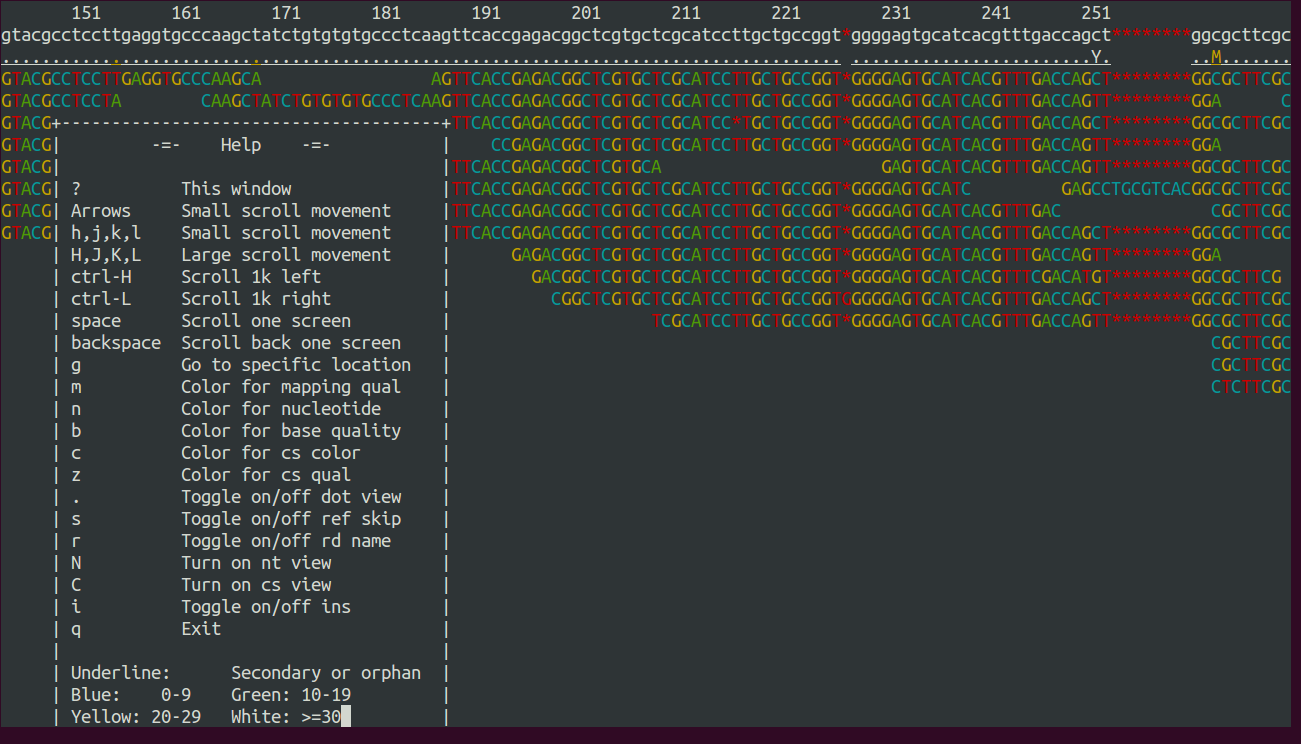
\includegraphics[width=14.5cm]{tview.png}
\caption{\label{fig:tview}Screenshot of tview}
\end{figure}

\clearpage
\subsection{IGV: viewer with a graphical user interface}
\label{sec-3-2}
I bet that many of you prefer to look at the alignment in a graphical
user interface. A decent free alignment viewer is \href{https://www.broadinstitute.org/igv/}{igv}, the Integrative
Genomics Viewer (see Fig. \ref{fig:igv} for a screenshot). Once you have
registered, you can launch the program with Java Web Start. We can't
promise that this works well in the course, since everything that
relies on a graphical user interface can be quite slow when using a
remote connection. Thus, you might want to download the required files
(deduplicated SAM file and reference genome) and try out igv on your
private computer. The interface is pretty much self-explanatory. To
look at the alignment, you first need to load a genome and then add
the mapped, sorted and indexed bam file.



\begin{figure}[htb]
\centering
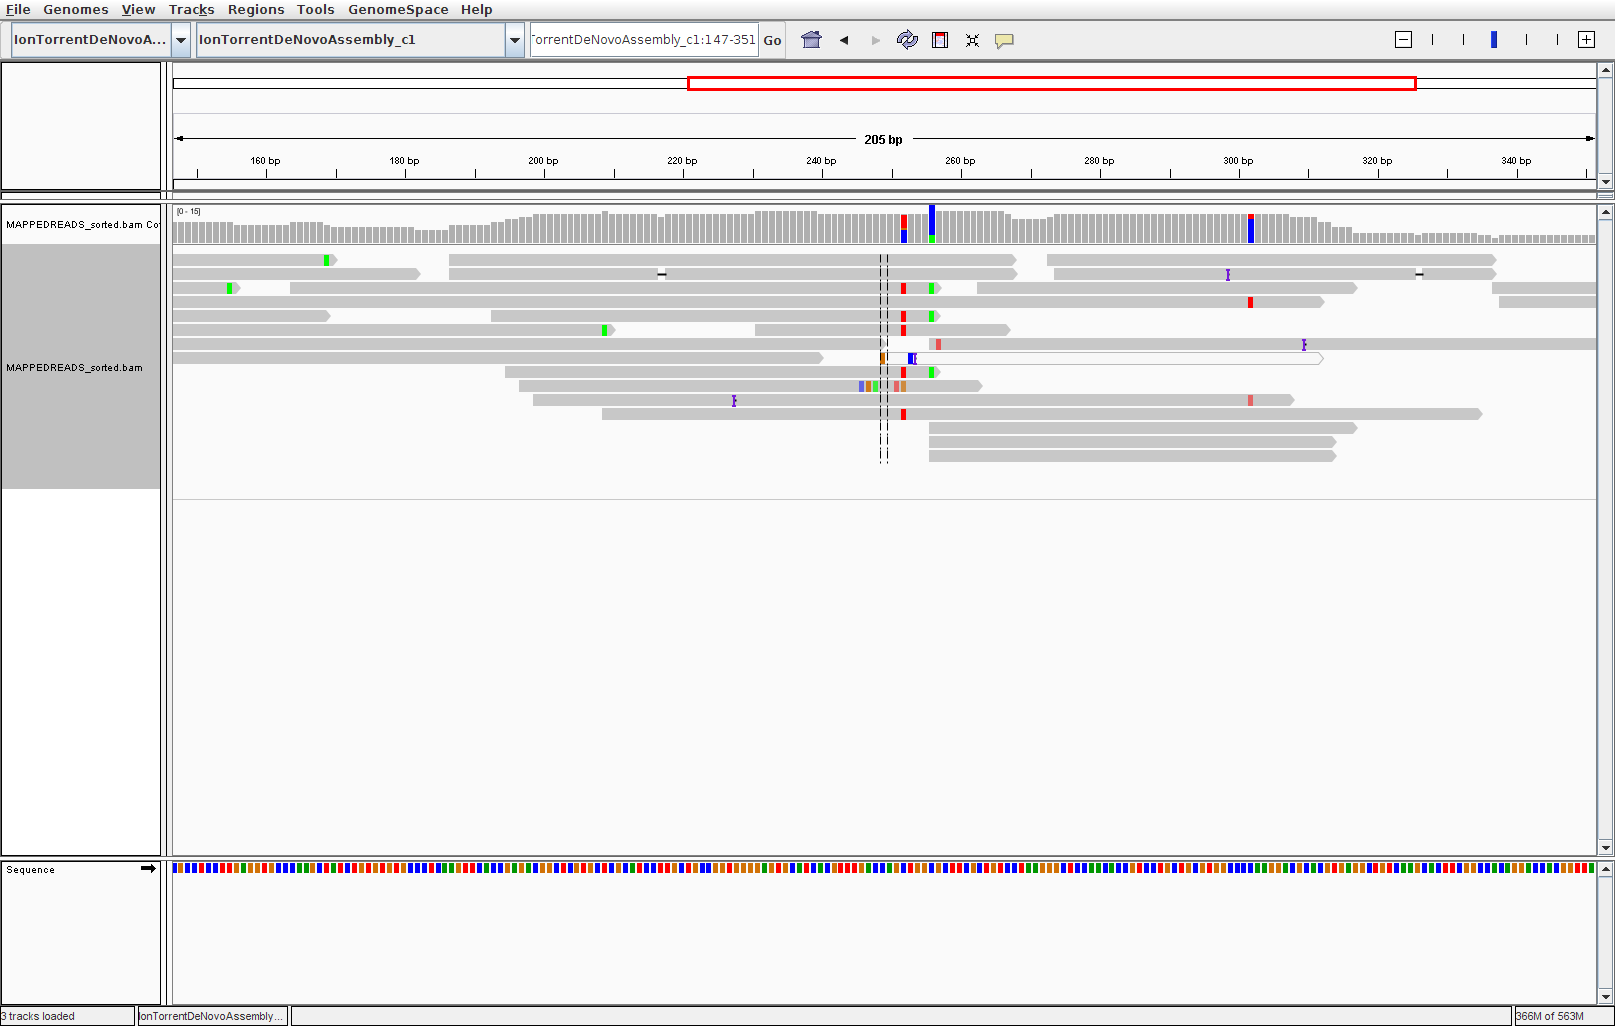
\includegraphics[width=17cm]{igv.png}
\caption{\label{fig:igv}Screenshot of igv with reads aligned to a reference and colored mismatches}
\end{figure}

\clearpage
\section{BONUS: SNP calling with samtools mpileup and bcftools}
\label{sec-4}
A widely used tool to identify sequence variants is \texttt{samtools
mpileup}. See \href{http://samtools.sourceforge.net/samtools.shtml}{here} for an overview of its options. The tool \texttt{samtools
mpileup} defaults to creating a pileup file, which summarizes aligned
base calls in text format (see here for a detailed characterization of
a pileup file \url{http://samtools.sourceforge.net/pileup.shtml}). If you
call \texttt{samtools mpileup} with the \texttt{-u} or \texttt{-g} option, instead, the
output format is a vcf or bcf (compressed binary version of vcf) file;
vcf stands for 'variant call format'. Its format specifications are
described \href{https://samtools.github.io/hts-specs/VCFv4.2.pdf}{here} and summarized in Fig. \ref{fig:vcf}.

The first step for calling SNPs from your aligned and deduplicated
reads is:

\begin{minted}[fontsize=\scriptsize,bgcolor=lightgray,linenos]{sh}
samtools mpileup -g \
-f \
IonTorrentDeNovoAssembly_out\
.unpadded.fasta \
-q 20 \
-Q 20 \
-t DP \
-t SP \
MAPPEDREADS_dedup.bam  > MAPPEDREADS_dedup.bcf
\end{minted}

The chosen options are described on this \href{http://samtools.sourceforge.net/samtools.shtml}{page}. By setting the \texttt{-t SP} and
\texttt{-t DP} tags, samtools mpileup provides:

\begin{description}
\item[{\texttt{-t SP}}] per-sample Phred-scaled strand bias P-value
\item[{\texttt{-t DP}}] per sample read depth
\end{description}


To call SNPs from the bcf file, we use bcftools:

\begin{minted}[fontsize=\scriptsize,bgcolor=lightgray,linenos]{sh}
bcftools call -vm -V indels MAPPEDREADS_dedup.bcf >  MAPPEDREADS_variants.vcf
\end{minted}


Options:
\begin{description}
\item[{\texttt{-v}}] Output variant sites only
\item[{\texttt{-V indels}}] Skip indels
\item[{\texttt{-m}}] model for multiallelic and rare-variant calling
\end{description}


\begin{figure}[htb]
\centering
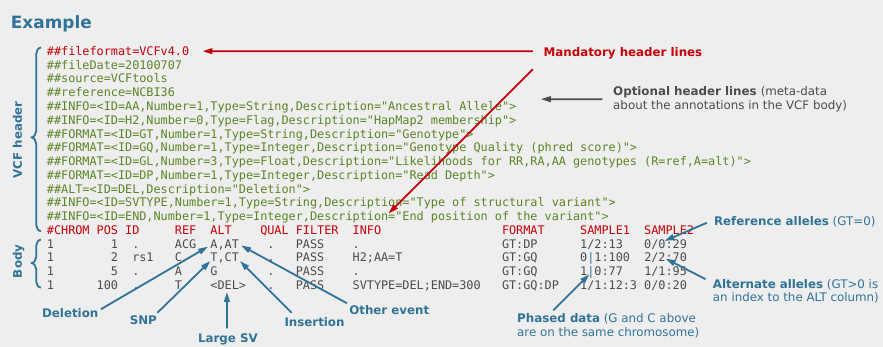
\includegraphics[width=17cm]{DanecekVcfFile.png}
\caption{\label{fig:vcf}VCF file overview from \href{http://vcftools.sourceforge.net/VCF-poster.pdf}{Petr Danecek}}
\end{figure}



To count how many SNPs were found, use the following command:

\begin{minted}[fontsize=\scriptsize,bgcolor=lightgray,linenos]{sh}
grep -v -c '^#' MAPPEDREADS_variants.vcf
\end{minted}

The option \texttt{-v} in combination with \texttt{\textasciicircum{}\#} excludes all header lines
that start with (\texttt{\textasciicircum{}}) the \texttt{\#}-sign. With the \texttt{-c} option, grep counts
the lines instead of writing them out.


To filter out SNPs that are low quality or covered by low depth, we
can use the \texttt{vcfutils.pl varFilter} that comes with samtools:

\begin{minted}[fontsize=\scriptsize,bgcolor=lightgray,linenos]{sh}
vcfutils.pl varFilter -d 5 -w 3 -Q 20  MAPPEDREADS_variants.vcf > MAPPEDREADS_variants_filtered.vcf
\end{minted}


Options used:
\begin{description}
\item[{\texttt{-d 5}}] minimum read depth of 5
\item[{\texttt{-w 3}}] SNP within 3 bp around a gap to be filtered. This may be
an alternative solution to re-alignment around indels
\item[{\texttt{-Q 20}}] minimum mapping quality of 20
\end{description}

Another useful option can be:
\begin{description}
\item[{\texttt{-1 0.0001}}] min P-value for strand bias (given the PV4-tag in the
vcf file). We obtained the PV4-tag by setting the \texttt{-t SP} tag in
\texttt{samtools mpileup}. This option filters out the SNPs that have a
strong strand-bias: SNPs that are supported by one strand and not
the other.
\end{description}


Count how many SNPs are left after filtering

\begin{minted}[fontsize=\scriptsize,bgcolor=lightgray,linenos]{sh}
grep -v -c '^#' MAPPEDREADS_variants_filtered.vcf
\end{minted}

The SNPs can be visualized with IGV. For this, we first need to
compress and index the vcf files: 

\begin{minted}[fontsize=\scriptsize,bgcolor=lightgray,linenos]{sh}
bgzip -c \
MAPPEDREADS_variants_filtered.vcf \
> MAPPEDREADS_variants_filtered.vcf.gz

tabix \
-p vcf \
MAPPEDREADS_variants_filtered.vcf.gz
\end{minted}

Open IGV and load the indexed bam file and the indexed vcf file.
Emacs 24.3.1 (Org mode 8.3beta)
\end{document}